\chapter{Requirement analysis}\label{chapters:analysis}

% Uvod do teto kapitoly
This chapter summarizes expectations for the application in a form of requirements. The requirements are analyzed and the solution is proposed in the next chapter with focus on formal description of the framework.

\bigskip

% Co tady dat klicove stakeholdery?

As a \textbf{stakeholder} we would consider data analyst, programmers, or at least people interested in the area of data-modelling, as the typical use-case of the application is (i) to design schemas for a large system of interconnected subystems or modules, or (ii) to design a recommendation for publishing data. Both these use-cases were described in the introduction of this chapter.

Because of the knowledge in the area of data modelling of all the stakeholders, we may have the UI of the application for those users more technical as the intent of the application and all the operations may be intuitive for them.

Nevertheless, the basic functionality does not require the advanced knowledge in the fields mentioned above, therefore we propose an "expert mode". User will be asked whether he or she feels to be an expert in the field which would make available more advanced features of the application, while keeping the UI simple for those interested in basics of data modelling.

\bigskip

\begin{requirement}
A user shall be able to easily derive a general schema structure from the existing ontologies and then translate the structure into different known schema languages, such as JSON Schema, XSD and CSVW Schema and it shall be possible to add support for others easily.
\end{requirement}

The basic idea behind this requirement was already explained in the introduction chapter. From an ontology, which specifies the relations between things from a real world, should be possible to easily select relations and things that will describe a schema. The schema then describes a structure of data that represents those things.

\smallskip

Our goal is to design a model capable of describing a data schema of common data formats. This schema will be used as a mapping from the ontology to the desired structure. The structure model must be robust enough to support different formats, as we want to use the same model for different formats.

Data serialization is a process of storing object state in a format that can be read back later. There are many different models for serialization with the most known as:
\begin{itemize}
    \item \textbf{Hiearchical model} stores data in a tree-like structure. This was one of the most common model for serialization of data in past few decades as it was easy to understand and interpret. XML and JSON are examples of formats that use this model.
    \item \textbf{Relational model} uses tables to store data. Each column is defined in advance and rows denotes the entities. Rows may point to rows in other tables to link data.
    \item \textbf{Graph model} represents data in graph.
\end{itemize}

% Tady vlastne rozeberu, ze ok, je to ve stromove strukture. No a ted jak by mela vypadat a proc zrovna takhle. Zamerim se na asociaci na tridu, ktera je na jedom radku. Nejaky obecny kocept, jak se treba vydat i do budoucna a jake jsou alternativey, napriklad ve srovnani s xcase, kde to bylo stromove.

As our main intent is to support JSON and XML, we will use the first type of model to represent data in our general format. The translation from that format to individual schemas in hiearchical model would be implicit.

Supporting translation from the general schema in hiearchical model to other formats in relational and graph model should be possible in a limited way\footnote{That means we may not be able to reverse translation from specific schema to the general schema or it may not be possible to use the full power of the given specific schema. However, this is not important to us as our target is support for basic use-cases.}, which is sufficient and is in accordance with the requirement to have one general schema. The last type of model is not even necessary to generate as we use the ontology that is already in graph model, hence we can use directly the ontology as the schema to validate our data.

To make the model applicable in practice, we need to support advanced format-specific constructs as well. Those constructs should not forbid us to use the model for other formats if possible and should be easily adaptable to new formats.

Because of a vast majority of different schema languages, we cannot have too strict requirements on the model or the ontology, as some schemas may not require all the information or may be too simple. This pushes us to define these two concepts in the most elementary way.

\begin{figure}\centering
    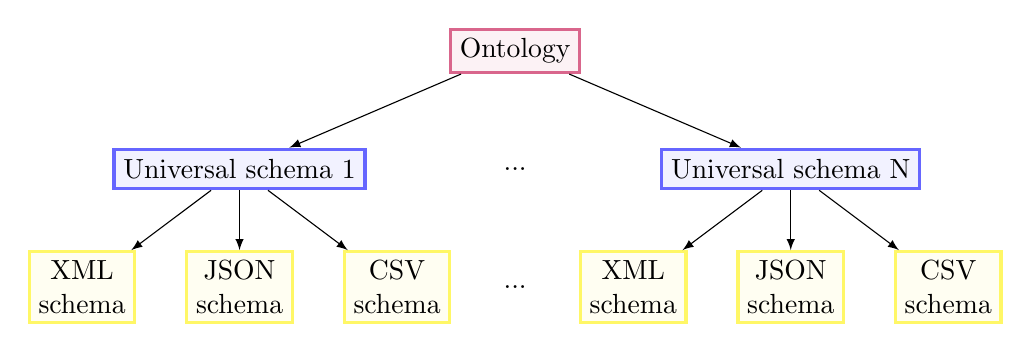
\begin{tikzpicture}[
        squarednode/.style={rectangle, draw=blue!60, fill=blue!5, very thick, minimum size=5mm},
        schema/.style={rectangle, draw=yellow!60, fill=yellow!5, very thick, minimum size=5mm},
        ontology/.style={rectangle, draw=purple!60, fill=purple!5, very thick, minimum size=5mm},
    ]
        %Nodes
        \node[ontology] (ontology) at (0,0) {Ontology};

        \node[squarednode] (schema1) at (-3.5,-1.5) {Universal schema 1};
        \node (psmDot) at (0,-1.5) {...};
        \node[squarednode] (schemaN) at (3.5,-1.5) {Universal schema N};

        \node[schema,align=center] (xml1) at (-5.5,-3) {XML\\schema};
        \node[schema,align=center] (json1) at (-3.5,-3) {JSON\\schema};
        \node[schema,align=center] (csv1) at (-1.5,-3) {CSV\\schema};

        \node (psmDot) at (0,-3) {...};

        \node[schema,align=center] (xmlN) at (1.5,-3) {XML\\schema};
        \node[schema,align=center] (jsonN) at (3.5,-3) {JSON\\schema};
        \node[schema,align=center] (csvN) at (5.5,-3) {CSV\\schema};

        %Lines
        \draw[-latex] (ontology) -- (schema1);
        \draw[-latex] (ontology) -- (schemaN);

        \draw[-latex] (schema1) -- (xml1);
        \draw[-latex] (schema1) -- (json1);
        \draw[-latex] (schema1) -- (csv1);

        \draw[-latex] (schemaN) -- (xmlN);
        \draw[-latex] (schemaN) -- (jsonN);
        \draw[-latex] (schemaN) -- (csvN);
    \end{tikzpicture}
    \caption{Diagram showing the core workflow behind the data modelling from a ontology. User can create universal schemas (blue rectangles) from the ontology from which are created traditional data schemas, such as XSD, CSV Schema or JSON schema.}
\end{figure}

%Tady pozadavek na tu strukturu, tedy ze bude stromova, do radku chceme sjednocovat asociace a celkove to ma byt barevne a ikonkove odlisene.



We have already stated that a hiearchical model is preferred for the internal universal schema as it can be used to create also CSVs, that are in a relational model. Although we havent specified how the structure should look like, there might be references, as the schema may point to other schemas. This

Previous tools \textit{xCase} and \textit{eXolutio} used full graph editor instead of simplier list to show and modify the universal schema. In the general case, users may benefit from the graph view if the schema refers to another schema multiple times, because this can be easily denoted in the graphical interface (see \autoref{analysis/difference-between-graphical-and-hiearchical}). On the other hand, schemas such as XML or CSV often depends on the order of its elements. This is easier to capture in the hiearchical model as all the items are in the list which has some order implicitly.

\begin{figure}\centering
    \begin{subfigure}{.5\textwidth}
        \centering
        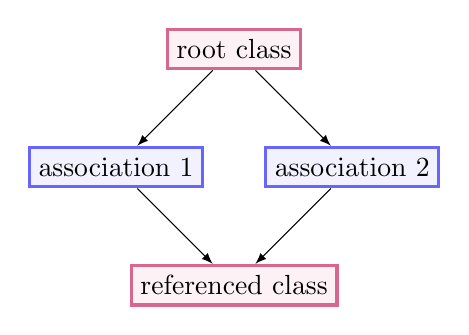
\begin{tikzpicture}[
            squarednode/.style={rectangle, draw=blue!60, fill=blue!5, very thick, minimum size=5mm},
            schema/.style={rectangle, draw=yellow!60, fill=yellow!5, very thick, minimum size=5mm},
            ontology/.style={rectangle, draw=purple!60, fill=purple!5, very thick, minimum size=5mm},
        ]
            %Nodes
            \node[ontology] (root) at (0,0) {root class};

            \node[squarednode] (a1) at (-1.5,-1.5) {association 1};
            \node[squarednode] (a2) at (1.5,-1.5) {association 2};

            \node[ontology] (ref) at (0,-3) {referenced class};

            %Lines
            \draw[-latex] (root) -- (a1);
            \draw[-latex] (root) -- (a2);
            \draw[-latex] (a1) -- (ref);
            \draw[-latex] (a2) -- (ref);
        \end{tikzpicture}
        \caption{Graphical representation}
      \end{subfigure}%
      \begin{subfigure}{.5\textwidth}
\begin{Verbatim}[commandchars=\\\{\}]
{\color{purple!60}root class}
  {\color{blue!60}- association 1}
    {\color{purple!60}- referenced class}
  {\color{blue!60}- association 2}
    {\color{purple!60}- referenced class}
\end{Verbatim}
        \caption{Hiearchical representation}
      \end{subfigure}

    \caption{Figure showing a schema referencing the same subschema twice, essencially creating a cycle in unoriented graph. Two different representations are shown - graph and hiearchical.  The former one shows that both associations refer the same subschema, which later representation can not show.}
    \label{analysis/difference-between-graphical-and-hiearchical}
\end{figure}


\begin{requirement}
    The application shall create a supporting documents to the generated schemas.
\end{requirement}

As the main goal of the application should be to generate schemas, we also need to create documentations to them, diagrams and examples. This requirement has already been explained in the example in the introduction chapter.

% Tady treba jeste s pluginama, mozna jako separatni requirment, aby se ta aplikace dala rozsirovat.

% Pozadavek na OFN?

\begin{requirement}
    \label{requirement:ontologies-on-the-web}
    As many ontologies are located on the web in formats like OWL, RDFs, UFO, etc., the application shall support reading them.
\end{requirement}

This has the following impacts:
\begin{enumerate}
    \item The ontology may \textbf{not always be available}. Unavailability should not forbid us from generating the schemas and making minor changes to them if those changes are not directly related to exploring the ontology.
    \item The concepts in the ontology may \textbf{point to another ontology} according to Linked Open Data principles.
\end{enumerate}

\begin{requirement}
    \label{requirement:pim-editing}
    The previous approach of creating the ontology directly in the application is not required, but there should be support for \textit{some} modifications.
\end{requirement}

\begin{requirement}
    The application shall support generating transformations between different data formats that conforms supported schemas and RDF representation.
\end{requirement}



% Necaskeho pozadavek na OR a hierarchii
% https://github.com/mff-uk/dataspecer/issues/95

\begin{requirement}
    It shall be possible to easily add more specific classes to the universal schema that extends the base class in a way that data, that conforms the resulting schemas, may contain either the base class, or one of its specialization.
\end{requirement}

\begin{showcase}
    We will start directly with an example. Suppose, that the warehouse also distributes foods besides the general goods. Food is of course type of good, but for storing purposes, it may have additional attributes, such as \textit{storing temperature}. When designing a schema that contains goods anywhere


\end{showcase}

This requirement impacts the application on two different levels. First, the universal schema model has to have constructs to represent the required problem and all generators shall understand them and generate a schema that corresponds to the intended result.

Generaly speaking, inheritance is a complex concept, that can be expressed in more simple way. Unfortunatelly, to make this pleasible for a user, we need to represent some things % such as association to class

% Analyza co vsechno se da udelat, co bude privetive a co ne. Rozeberu to na zakladni OR a include.

\section{Future requirements}

Following requirements in this section are analyzed and may have an impact on the final model that will be discussed in the next chapter. But due to its complexity, full implementation and analysis will be kept as authors future work and this thesis cover only the necessity to not introduce a technical debt.

\begin{requirement}
    It shall be possible to perform a top-down evolution of schemas and other documents from an ontology. The evolution shall be automatic, if possible, and shall also transorm the data that conform the given schemas. The application shall also deduce the changes from an ontology that does not support versioning.
\end{requirement}

Schema evolution is a large topic with many theoreticall issues.

% popis evoluce, priklady


%%%%%%%%%%%%%%%%%%%%%%%%%%%%%%%%%%%%%%%%%%%%%%%%%%%%%%%%%%%%%%%%%%%%%%%%%%%%%%%%

\begin{requirement}
    As there shall be a support for data transformations between different schemas, the data transfomations shall respect various ontology alignments to transform data between different ontologies. Alignments shall be created also during user modification of the ontology, between the modification and the original ontology.
\end{requirement}

\textbf{Alignment} as defined in TODO is a set of relations between entities \textit{usually} from different ontologies. These relations specify the semantic equivalence between the entities and create a mapping that can transform data from one ontology to another.

There are already well-known RDF predicates that can cover basic alignment. For semantically identicall entities, we may use \verb|owl:equivalentClass| or \verb|skos:exactMatch|. More usefull RDF predicate is \verb|rdfs:subClassOf| for more specific classes representing things.

The later one is already included in the previous requirement TODO. Subclasses (i) reuses attributes and associations from its parent class, but also semantically denotes, that (ii) the subclass can also be treated as "the parent class". The second point is an example of a simple ontology alignment.

\begin{showcase}
    % example with address
\end{showcase}
